\subsection{System, communication and adversary model}%
\label{adversary-model}

We provide a system model with various adversaries.
We provide three adversaries of varying strength for the protester and two for 
the witness.

\paragraph{The protester adversary}

There are three players: the protest participant (with identity) \(P\), a 
witness (with identity) \(W\) and the storage \(S\).
The adversary \(A\) controls \(W\) and \(S\).

\begin{definition}[Base protester adversary]\label{base-protester-adversary}
  The protester \(P\) and the witness \(W\) communicate.
  Each learn only the protocol data \(d_{P,W}(\cid, P)\) and when it happened 
  \(t_{P,W}\)\footnote{%
    Specifically, they do \emph{not} learn the real identities \(P\) and \(W\) 
    directly, only if those appear in the data \(d_{P,W}(\cid, P)\).
  }.
  The protester \(P\) communicates with \(S\), where \(S\) only learns 
  \(f(d_{P,W}(\cid, P))\), for some function \(f\), and the time of the 
  communication (\(t_{P,S}\)) but not the real identities.
  The adversary controls \(W\) and \(S\) and thus learns everything that they 
  do, but can additionally correlate what he learns from \(W\) and \(S\).
\end{definition}

This definition is illustrated in \cref{fig:system-model}.

\begin{figure}
  \centering
  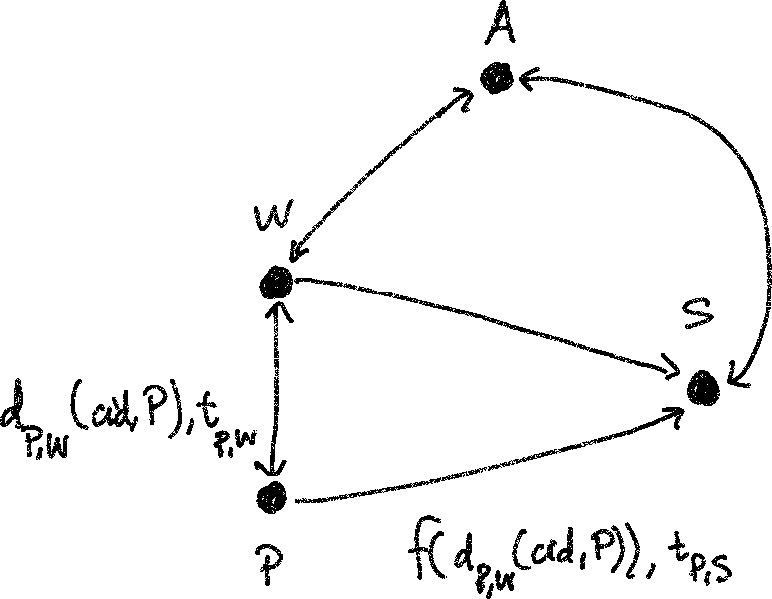
\includegraphics[width=\columnwidth]{system-model.png}
  \caption{\label{fig:system-model}%
    An overview of the system model.
    The protester with real identity \(P\) and witness with real identity \(W\) 
    communicate and each learn only the protocol data, \(d_{P,W}(\cid, P)\), 
    and the time it happened, \(t_{P,W}\).
    The protester submit some function of the protocol data \(f(d_{P,W}(\cid, 
      P))\) to the storage \(S\), who learns only that and the time it 
    happened, \(t_{P,S}\).
    Both the witness \(W\) and storage \(S\) are controlled by the adversary 
    \(A\).
  }
\end{figure}

We find \cref{base-protester-adversary} suitable when the protester and witness 
both move in a crowd and there is no way for the witness to decide exactly with 
whom he or she communicates with.
However, in some situations this might not be the case, \eg the crowd is not 
dense.
In these situations the witness will likely see the face of the protester.
We capture this by the following definition.

\begin{definition}[Stonger protester adversary]%
  \label{stronger-protester-adversary}
  The situation is the same as in \cref{base-protester-adversary}, but now the 
  witness \(W\) learns the protester \(P\)'s identity.
  (\(P\) will also learn \(W\)'s identity.)
  However, \(S\) still does not learn \(P\)'s identity.
\end{definition}

One reason to not allow \(S\) to learn \(P\)'s identity is that for this 
communication \(P\) has options, such as \ac{Tor}, for anonymous communication.
However, given a strong enough adversary, such anonymous communication might 
not be possible.
Hence the following definition.

\begin{definition}[Strongest protester adversary]%
  \label{strongest-protester-adversary}
  Everything is the same as in \cref{stronger-protester-adversary}, except that 
  now \(S\) also learns \(P\)'s identity.
\end{definition}

\paragraph{The witness adversary}

The players are still the same, but now the adversary controls other players.
In particular, the adversary controls the protester \(P\) and the storage 
\(S\).

\dots

